% Although we admit that the rat is bombarded by stimuli, we hold that his nervous system is surprisingly selective as to which of these stimuli it will let in at any given time. (...) Both strip-maps and comprehensive-maps may be either correct or incorrect in the sense that they may (or may not), when acted upon, lead successfully to the animal's goal. The differences between such strip maps and such comprehensive maps will appear only when the rat is later presented with some change within the given environment.
% Tolman

% \begin{savequote}[75mm]
% Do not become the archivist of facts. Try to penetrate to the secret of their occurrence, persistently search for the laws which govern them.
% \qauthor{Ivan Pavlov}
% \end{savequote}

\begin{savequote}[75mm]
The smallest group of facts, if properly classified and logically dealt with, will form a stone which has its proper place in the great building of knowledge, wholly independent of the individual workman who has shaped it
\qauthor{Karl Pearson}
\end{savequote}


\chapter{General Discussion}
\label{chap:results}

In the present chapter, we frame our results in the light of distinct theoretical frameworks to allow for their contextualization within a broad perspective.

\section{Reassessment of model predictions}
    In section \ref{sec:models} we have presented two algorithmic models that account for time learning, alas the SET and LeT. Here we try to assess predictions with respect to their time representations. 
    
    The LeT model is divisible into three components: 1. The "behavioral" states, that progress serially during each trial; 2. The connections between behavioral states and action decisions; 3. The possible action decisions. The temporal representation in this model is static during learning, because it is contained within the sequence of behavioral states. What is learned is the decision policy that the animal uses to guide behavior, i.e. when to act. In other words, it is like if the animal already has a clock, but needs to learn where (in the clock representation) an action is warranted.
    
    The SET model is very similar to LeT in its predictions, although their conceptualizations differ. The pacemaker and accumulator are analogous to the LeT behavioral states, in the sense that they offer a sequential representation of time that is present from the onset of the task. Moreover, SET's comparator serves the same role as the decision function, to guide behavior. Nevertheless, the biggest distinction between them can be traced to the memory module, which in the LeT model is explicitly distributed, while in the SET model is rather undefined - provided that it is able to persist. In the SET model, learning occurs by refining the long-term memory of the rewarded time, described by the mean of all rewarded time representations. 
    
    Alternatively to SET and LeT, models based on State Dependent Networks (SDNs) propose that the trajectories themselves can be learned \cite{goudar2018encoding}, as represented in figure \ref{fig:sdn_trajectories_training}. In such models, the time representation itself is sharpened by training, increasing the consistency between trajectories from distinct trials, as illustrated in figure \ref{fig:sdn_trajectories_training}. Because the population activity across trials becomes more consistent for each time point, it consequently becomes more reliable to predict time. Then, activity can be read out to guide a decision.
    
    \begin{figure}
        \centering
        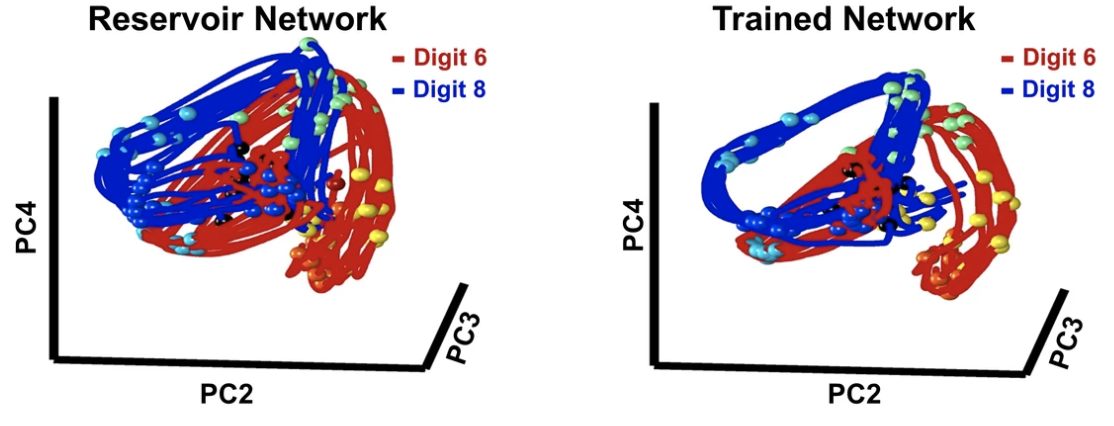
\includegraphics[width=.8\textwidth]{figures/sketches/sdn_trajectories_training.png}
        \caption[Activity trajectories in an artificial neural network]{Activity trajectories in an artificial neural network. In both cases, activity of a network is recorded in response to the same stimulus, with noise inputs added. In the left, untrained trajectories. In the right, trajectories for a neural network that has been trained to follow the trajectory without noise. Adapted from Goudar and Buonomano \cite{goudar2018encoding}}
        \label{fig:sdn_trajectories_training}
    \end{figure}

    % Trajectories are better able to tackle problems that involve complex patterns \cite{paton2018neural}, like motor responses \cite{}, but they involve more 
    
    Concerning our findings, the comparison of decoding performances during naivety and proficiency phases revealed distinct evolution patterns in the mPFC and Striatum. The Striatum presented results consistent with our hypothesis, exhibiting the absence of a neural representation at a naive stage, which later develops with training. In an opposite direction to this process, and in stark contrast to our expectations, the mPFC started with a time representation that decreased with training. We will leave aside for a moment the opposite trends we have found, and treat each one separately. 
    
    A robust time representation, possibly present in the mPFC at the beginning of training, could be assigned to either the behavioral states of the LeT model or the integrator of the SET. The same could be done for the Striatum activity in the trained stage. In either case we are assuming that the decision function is being learned parallel to the time representation, and that the representation changes that we see are not contained or explained by the models. The representation later presented in the Striatum would have to be learned in some way not described by the models. 
    
    We can also assign the time-dependent consistent activity we are measuring to the decision function component of either SET or LeT. In this case the degree of confidence in the reward increases with the passage of time, and the neural activity containing the confidence readout would present a time-dependent consistent activity. In this case, the measurements are not time representation in the algorithmic sense, but an epiphenomenal time-consistent activity. Epiphenomenal in the sense that it is a temporal consistency without causal role in time-locked activity, in the same way as the rush hour does not cause the work expedient to begin.

    In sum, the discussion encompassing SET and LeT models cannot properly account for the changes in time-consistency observed in the neural activity during training. We can, however, explain some of this changes by assigning the Striatum activity to the SDN's neural trajectory. The activity in the Striatum was unable to predict time early on, but showed enhancements with training, in a coherent fashion to the recurrent network by Goudar and Buonomano \cite{goudar2018encoding}.
    
    % Lets suppose, as a simplifying assumption, that the implementations of each one of LeT's components, as well as the trajectory, reside in neural activity measurable with electrodes. If we recorded from LeT behavioral states, we would not perceive any big change during training, and would probably be able to detect a time representation since the beginning. Alternatively, if we recorded from the decisional component, we would only be able to detect the 

    % We just presented an algorithm learns a time representation or only the decision function. has consequences on the tasks it can solve. 

\section{Striatum and medial Pre Frontal Cortex show opposite trends}
    The models of timing, as currently proposed, may offer only partial descriptions to our findings. In particular, our unexpected findings of a decrease in classifier performance with training in the mPFC, in contrast to an increased performance in the Striatum, poses a challenge as to be described in the terms of timing models.
    
    In attempt to gain a better understanding on these results, our group developed a follow-up experiment capable to provide some causal evidence. Specifically, the mPFC of rats was experimentally inactivated and the same DRRD task was performed. The inactivations impaired animals only during learning, and not during proficient performance (G Chiuffa et al., in preparation). This additional finding supports our present analysis, and expands it to causal consequences: there is an initial involvement of the mPFC that later decreases or vanishes.
    
    The mPFC has been shown both to encode task-relevant information during learning \cite{kaplan2017role} and to decrease this encoding after learning \cite{schuck2015medial}, which is in agreement with our results. Moreover, while disruption of PFC's dopamine receptors was found to impair associative learning in some tasks, it was found not to impair performance of learned associations \cite{puig2012role, puig2014prefrontal}. Additionally, the differential engagement of the cortex in learning but not in task execution has been shown also in the motor cortex \cite{kawai2015motor}. 
    
    This set of findings motivates the development of a model where the cortex "tutors" the Striatum, which is the responsible for driving performance after learning \cite{murray2017learning}. Accordingly, the Striatum has been shown to play a role in associative learning \cite{li2011differential,liljeholm2012contributions}, specially with regard to the performance of overlearned behaviors \cite{smith2013dual}. This role for the Striatum is also compatible with our results.
    
    We have searched in the timing literature for theoretical accounts that made sense of our findings, but did not find any explicit accounts for corticostriatal dependency changes. We next discuss our findings through a framework for learning that explicitly accounts for dependency changes with learning, called dual-process. 
    
\section{Observed patterns are consistent with dual processes}
    % With respect to mPFC importance in learning and not performance, this seems to be dependent, in humans, on the specific sub-region being evaluated. Studies on the vmPFC's, in the field of fear extinction, point out that it is necessary to retain learning \cite{phelps2004extinction}, and it seems also necessary to performance in gambling tasks \cite{rogalsky2012risky}. Distinctly, dmPFC's role has been verified to bolster learning but not performance \cite{balleine2007still}, mirroring the mPFC results from our group.
    An influential perspective for learning is the dual process framework. As described in section \ref{sec:learning}, it consists in a goal-directed system and a habitual system. Nevertheless, the potential contributions of such perspective in the context of timing have been rarely explored yet.
    
    Through the lens of instrumental learning, it could be inferred that learning in our DRRD task is first dominated by the flexible system, until it rapidly changes dependencies to the habitual system. In accordance with this possibility, a study found that initial performance in a T-maze task was dominated by the goal-directed system, as it was flexible to changes at the rewards. In turn, overtraining made the performance resistant to reward devaluation and dominated by habit \cite{smith2013dual}. This findings illustrate a general tendency of learning according to the dual process framework, although the speed in which this dependency changes occur varies depending on the task.
    
    Moreover, contrasting evidence to our findings come from a study using a different interval timing task. It was found that, using the same time scale as our, the mPFC was still engaged even after 10 learning sessions \cite{narayanan2006reversible}. Such differences could be expected in instrumental learning if either their task is more complex than ours, or their reinforcement schedule is more reliable than ours \cite{dickinson2015instrumental}. However, neither option provides a clear explanation, since comparisons are not straightforward.
    
    % \subsection{Previous accounts for dual process in timing}
        An account of dual-process in timing was presented by Lewis and Miall in a meta-analysis of fMRI timing studies in humans \cite{lewis2003distinct}. They proposed three dimensions that, in tandem, could split tasks into two groups with distinct neural substrates. The first group is Automatic Timing, dependent on motor and sensory circuitry such as Anterior Cingulate Cortex, primary Sensory Cortex and the Supplementary Motor Area. The second is Cognitively Controlled Timing, dependent on regions of the Pre Frontal Cortex and Intra Parietal Sulcus, among others. The dimensions proposed, which suffice to distinguish the two task groups, were the following:
        
        \begin{enumerate}
            \item \textit{Interval size}. Long intervals tend to require cognitively controlled timing.
            \item \textit{Presence of movement}. Movement eases the use of automatic systems for timing.
            \item \textit{Continuity/predictability}. When intervals are measured in a repeating cycle or in a predictable pattern, less attention is required by the task and thus it may be tackled by the automatic system.
        \end{enumerate}
        
        The dimensions they proposed map into those recently proposed by Paton and Buonomano \cite{paton2018neural}, that are Short/Long, Motor/Sensory, and Simple/Pattern. The major distinction between the two approaches is that while Paton and Buonomano treat the dimensions independently, Lewis and Miall propose a composite dimension, ranging from automatic to cognitively controlled mechanisms. Hence, instead of the eight possible combinations of the three dimensions, Lewis and Miall propose there are two important subspaces.
        
        Under the view of instrumental learning, we would expect that, given enough training, any task would be controlled by the automatic system. Nevertheless, this effect is dependent on task characteristics, hence some types of tasks would still be controlled by the goal-directed system, while others already would be processed automatically, provided the same amount of training. Therefore, according to Lewis and Miall, for each amount of training, there would be a two-dimensional surface (analogous to a hyperplane) separating the tasks that are automated from those that are still flexible, in the three-dimensional space proposed by them.
        
        The timing literature offer some accounts for automatic timing, but the specific boundary between automatic and non-automatic timing is far from established. The dual process account proposes that there is in fact no clear boundary when considering only the interval size dimension. Giving an illustrative example, it is like asking for the temperature at some time of the day without specifying neither the location in earth nor the season: the deviation is so large that the estimation is poorly informative. However, if we fixate other important variables, in our case the predictability, movement, and amount of training, we can potentially reduce deviation around the boundary.
        
        One challenge in reconciling the dual-process for timing with the framework of learning concerns the role of predictability. In instrumental learning, increasing reliability of the reward makes the goal-directed system more dominant in behavior. On the other hand, in Lewis and Miall's proposal, predictability reduces the need for attention, thus making the automatic system dominant. The apparent contradiction rests on a subtle distinction between their predictabilities. On the one hand, the former refers to predictability of reward given responses, so as to establish Response-Outcome (R-O) associations. In turn, the latter refers to state predictability, in the sense that sensory evidence is less noisy, and it rests upon the State-Response (S-R) associations.
        
    % \subsection{Associations and timing in the light of dual processes}
        To relate better this ideas to the timing domain, we delve deeper into the specific literature of time learning. While time is understood as an essential dimension for learning associations \cite{balsam2009temporal,kirkpatrick2016associative}, it may actually be either an attribute encoded in the associations \cite{molet2014timing} or a precursor to the learning of associations \cite{balsam2002timing}. Our original hypothesis is in line with the first case, as we expected time representations to develop during learning, and we found the activity in the Striatum to be consistent with this statement. On the other hand, our results for the mPFC are more closely in line with the precursor perspective \cite{balsam2002timing}, because time representation in that region seems to be present even when task performance is poor. 
        
        Bridging back to the timing models discussed above we find that, in SET and LeT, time is taken as a precursor to learning associations. In LeT this claim is made explicit: the association links between decisions and already-developed time representation are strengthened with training and rewarding. In turn, SDN models present mechanisms for learning the time representation, but do not provide a straightforward definition for potential associations to decisional processes. 
        
        % We argue below that it is possible to understand S-R associations for timing tasks as a kind of SDN's time representation. % Will we manage to do it? otherwise remove this
        
        
        
        % Let's designate the stimulus as the sensory information which is collected along time, such as a light that flashes for some duration, a sound, silence, heartbeats, some combination thereof, etc. This regular sensory information, embedded in a deeply changing sensory environment and internal contexts, generates neural activity that is diverse. To The animals' nervous systems uses 
        
        
        
        % In the stimulus-response
        
        % There are two learning process occurring simultaneously: the time representation (in the form of behavioral states), and the decision function (in the connections between states and rewards). A flexible and costly representation seems to be present from early on, and reward predictability makes possible to quickly learn policies, thus making the cognitive system more reliable for guiding behavior. The same reward predictability does not affect as much the policies of the automatic system, since they are not dependent on the Response-Outcome associations.
    
        % General state predictability, in the sense of a less noisy environment, probably enables easier training for the neural trajectories used for representing time in the automatic system. If this 
        

% The dissociation between timing and other aspects of behavior is a constant challenge in the present day \cite{kirkpatrick2016associative}.

%Reinforcement learning theories are central to the current understanding of learning processes and decision making in general, specially in the presence of rewards \cite{dayan2008decision, dohmatob2017dark, niv2016reinforcement}, and the PFC and Striatum are key areas in this framework \cite{dayan2008decision}, the PFC in relation to the , and the striatum 

%The representation of all the world's complexity into an well defined state space is essential to reinforcement learning \cite{mnih2015human}, and when information is not observable, the representation of the task state is supposed to be the role of the OFC \cite{wilson2014orbitofrontal}. The OFC may encode state information even when it is not important for behavior, and is proposed to disambiguate between task states that are perceptually similar but conceptually different, by encoding information about hidden variables \cite{schuck2016human}. While some state variables may be accounted for in other areas of the brain, non-observable task information may have their encoding only at the OFC, as shown in experimental works where a rats responded normally to tasks with explicit-signaled states, but showed deficits when task states were unobservable \cite{wikenheiser2016over}. In Reversal Learning and Delaying Alternation tasks, a Reinforcement Learning algorithm with a single state has similar results to OFC damaged rats \cite{wilson2014orbitofrontal}.

% niv2016reinforcement

% Time may be represented in the brain in the form of temporal maps \cite{kirkpatrick2016associative, fernandes2017episodic}, and its appearance in behavior 

%%%%%%%%%%%%%%%%%%%%%%%%%%%%%%%%%%%%%%

% Science is far from a perfect instrument of knowledge. It's just the best we have - Carl Sagan
\section{Limitations}
    It is common to 1) equate a classifier's performance with the presence of information in the neural activity, and even further to 2) believe that if information is present, then the animal has access to it  \cite{king2014characterizing}. 
    
    Firstly, the classifier's performance is not equal to the presence of information, it only \textit{implies} the information, meaning that the absence of prediction is possible even when there is information in the neural activity, for instance when the classifier is too strongly regularized. In the case that a classifier has been carefully tuned, and even so remained with a poor performance, we still have no way of knowing whether the region truly lacks information, or if information is concealed in hidden states such as presynaptic sensitivity, or internal states of the cells. Most of our discussion rests upon the implicit assumption that the only representation that is of interest to us is the neuronal activity, whilst changes in decoder performance could also be explained as representation shifts from activity states to hidden states, without entailing representation decay. 
    % although if we compare the same set of cells through time, we can have increased confidence in activity \textit{changes} and \textit{comparisons}.
    
    Secondly, classifiers can be powerful enough to extract meaning from information in a raw form, that will still be processed downstream \cite{king2014characterizing}. As an example, if we record enough cells from the primary visual cortex, we may be able to decode, given a strong classifier, the identity of different objects being seen, an information that is only encoded in higher visual areas. 
    
    The present study, by relying on comparisons across the same set of neurons, tackles the question as to whether the representation captured at one point is stronger or less variable than at other point. Most of our discussion rests upon the implicit assumption that the only representation that interests us is the one we have the capacity to measure, the neuronal activity. This assumption is not only ours \cite{bakhurin2017differential}, but is a single share of all possible representations including neuronal internal states and more. A recent article shows, for example, a case where accumulation of evidence is operated by the Glia \cite{mu2019glia}. If such mechanism was also used for the accumulation of time, it would not be captured by our data and neither by our analysis. 
    
    Although our group has pharmacological evidence that qualitatively agrees with the classification results, we have no conclusive evidence that the changes in classifier performance are in any way causally related to the changing regional dependencies. Moreover, we suppose activity will change similarly in different animals, implicitly assuming that animals employ the same strategies, at least with respect to time representation. The behavioral responses found here do not provide support for this assumption, since both the rolling mean and structure of peak responses are highly variable, but since these differences can also originate on the decision making, motor execution, or strategy of learning, they do not imply different strategies of time representation.


%%%%%%%%%%%%%%%%%%%%%%%%%%%%%%
% Representations

% Representations are generally hierarchical and nested \cite{seth2016active}. From single neurons to populations, the representations of sensory stimuly follow modality specific mechanisms \cite{}, and get farther from the primary cortices for more complex stimuli. Taking vision as an example: while angles of light sources are processed in V1, motion is processed in the MT region in the parietal cortex, and object identities in area V4 \cite{deyoe1988concurrent}. The same occurs in the motor domain \cite{hamilton2007motor,fernandes2017episodic}: while simple movements are traced to the M1 area \cite{graziano2016ethological}, complex movement patterns can be encoded in the supplementary motor area \cite{nachev2008functional}. 
%% Colocar imagem da hierarquia
% In the example of vision, the simplest representations are angles of light sources in V1, which resemble independent components of natural scenes \cite{bell1997independent}, making them an efficient representation for natural scenes. Representation of correlated edges, such as angles and contours take place at V2 \cite{ito2004representation, lee2008sparse}. What constitutes these simplest representations, present in the lowest level of the hierarchy, is specific for the modality being discussed, and it doesn't necessarily follow common sense \cite{}. While in the visual domain the simplest cortical representations are straight edges or bars \cite{bell1997independent}, in the motor cortex they are evolutionarily relevant movements like hand-to-mouth \cite{graziano2016ethological}. In the time domain, interoception modulation of interval timing \cite{pollatos2014interoceptive, tomasi2014dissecting}, points bodily states as one basis for interval timing \cite{bueti2011physiological, wittmann2010accumulation}, while other studies 
% They may be unusual basic operations in the sense that they dont f \cite[p.~3-4]{von2012computer}
% In higher levels of the hierarchy, representations develop invariances \cite{}

%The orbitofrontal cortex (OFC) or ventromedial frontal cortex (vmPFC) is one critical structure involved in emotion processing and decision making \cite{bechara2000emotion}. Damage to this structure may impair decision making both in social and personal domains, and is associated with impulsive and disinhibited behavior \cite{berlin2004impulsivity}.

% The taxonomy proposed is thorough in terms of Marr's levels. For each dimension, Paton and Buonomano characterize the existence of distinct computational requirements for each side. They discuss families of algorithms that are best suited for each, as well as associated neural regions and correlates. On the other hand, they focus on the implementation, with only marginal attention to the computational and algorithmic levels by themselves.
